\begin{surferPage}{巴斯六次曲線}
1996年,沃爾夫·巴斯(Wolf Barth)構造了這個六次曲面。巴斯六次曲面有65個奇異點。傑夫(Jaffe)與盧德曼(Ruberman)後來證明了巴斯六次曲面是奇異點最多的六次曲面——所以巴斯的世界紀錄是無懈可擊的!
巴斯曲面的出現對人們來說是一個巨大的驚喜,因為曾經在相當長的一段時間裡,人們誤以為六次曲面只能有 $64$ 個奇異點。
巴斯曲面具有一個非常好的性質:二十面體對稱性。下圖展示的是一個二十面體以及它的一個對稱平面。

  \begin{center}
    \vspace*{-0.1cm}
    \begin{tabular}{@{}c@{\ \ }c@{\,}c@{}}
      \begin{tabular}{@{}c}
        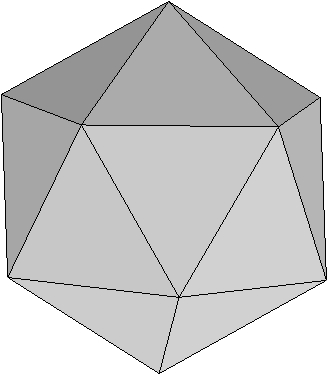
\includegraphics[width=1.4cm]{./../../common/images/icosah}
      \end{tabular}
      &
      \begin{tabular}{@{}c}
        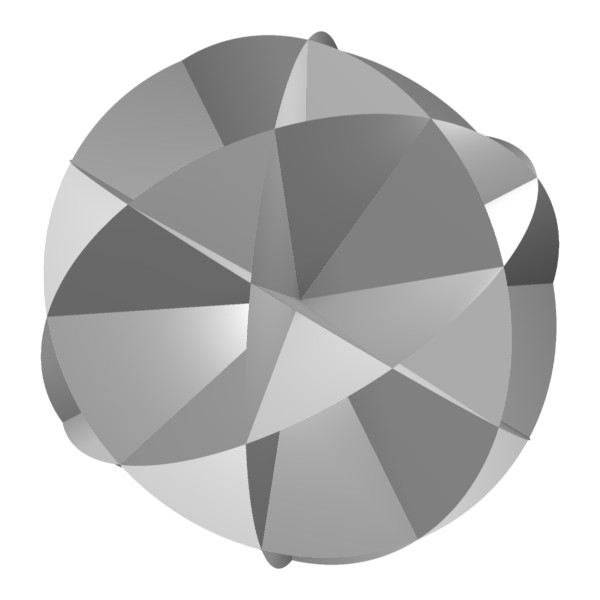
\includegraphics[width=1.4cm]{./../../common/images/barth_sextic_planes}
      \end{tabular}
      &
      \begin{tabular}{c@{}}
        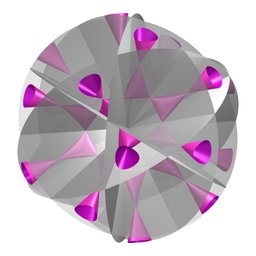
\includegraphics[width=1.4cm]{./../../common/images/barth_sextic_and_planes}
      \end{tabular}
    \end{tabular}
  \end{center}
  \vspace*{-0.1cm}

巴斯六次曲面滿足方程 $P_6 - \alpha K^2=0.$ 其中 $P_6$表示六個對稱平面, $K=x^2+y^2+z^2-1$ 是單位球面,並且
    $\alpha=\frac{1}{4}(2+\sqrt{5})$.
\end{surferPage}
